
\subsection{MNIST}
MNIST consists of a curated set of grayscale images (28x28) depicting handwritten digits.
The dataset is split into 60.000 training samples, 10.000 validation and 
10.000 testing samples. For this set, the approach of \cite{DBLP:journals/corr/abs-1202-2745} using CNNs is the best  model with a 0.23 error rate (23 out of 10.000 digits not recognized correctly).
We start our experience with the reference Theano model for MNIST which achieves 0.82 error rate. Its configuration is shown in Table\ref{fig:cnn1}
\subsubsection{CNN Model 1}
\begin{table}[h!]
\centering
\begin{tabular}{@{}rlll@{}}\toprule
Layer & Type & Maps and neurons& Kernel size \\ \midrule
0 & input & 1 map of 28x28 &\\
1& convolutional & 20 maps of 24x24 & 5x5\\
2 & max pooling & 20 maps of 12x12 &  \\
3 & convolutional & 50 maps of 8x8& 5x5 \\
4 & max pooling & 50 maps of 4x4&  \\ 
5 & fully conntected& 500 & \\
6 & fully conntected & 2 neurons & \\ \bottomrule
\end{tabular}
\caption{CNN Model 1 for MNIST}
\label{fig:cnn1}
\end{table}

We decompose the filter map from the first convolutional layer. From the theoretical point of view, according to Table \ref{table:rank}, we have a compact tensor $R^{20\times 5 \times 5}$ with a typical rank of 20 or 21, so we expect a very good aproximation for a rank in that range. 
Fig\ref{fig:cnn1fitness}a shows how well is the approximation with varying rank from 4 to 16 in steps of 2 on the $x$ axis and the fit on the $y$ axis (100 corresponds to perfect fit). As expected, the fit is almost perfect for high ranks and decreases afterwards.

Using separable filters, we obtain a theoretical speedup for convolutional layer 1 if $K<< \frac{Jd_{1}d_{2}}{J +d_{1}+d_{2}} = \frac{20\times 5\times 5}{20 + 5 + 5} = 16.66$. Fig\ref{fig:cnn1time}a shows the time improvements using separable filters. The blue line represents the time per layer using non separable filters. In our implementation, the separable filters give a speedup for any rank, as the red curve is below the blue one. 
We note that theoretically using non separable filters (blue line) and using separable filters with rank 16 should have given the same running time. The reason for the difference is due to implementation details and it is a language specific artifact.

\begin{figure}[h!]
  \centering
  \begin{subfigure}[b]{0.40\textwidth}
   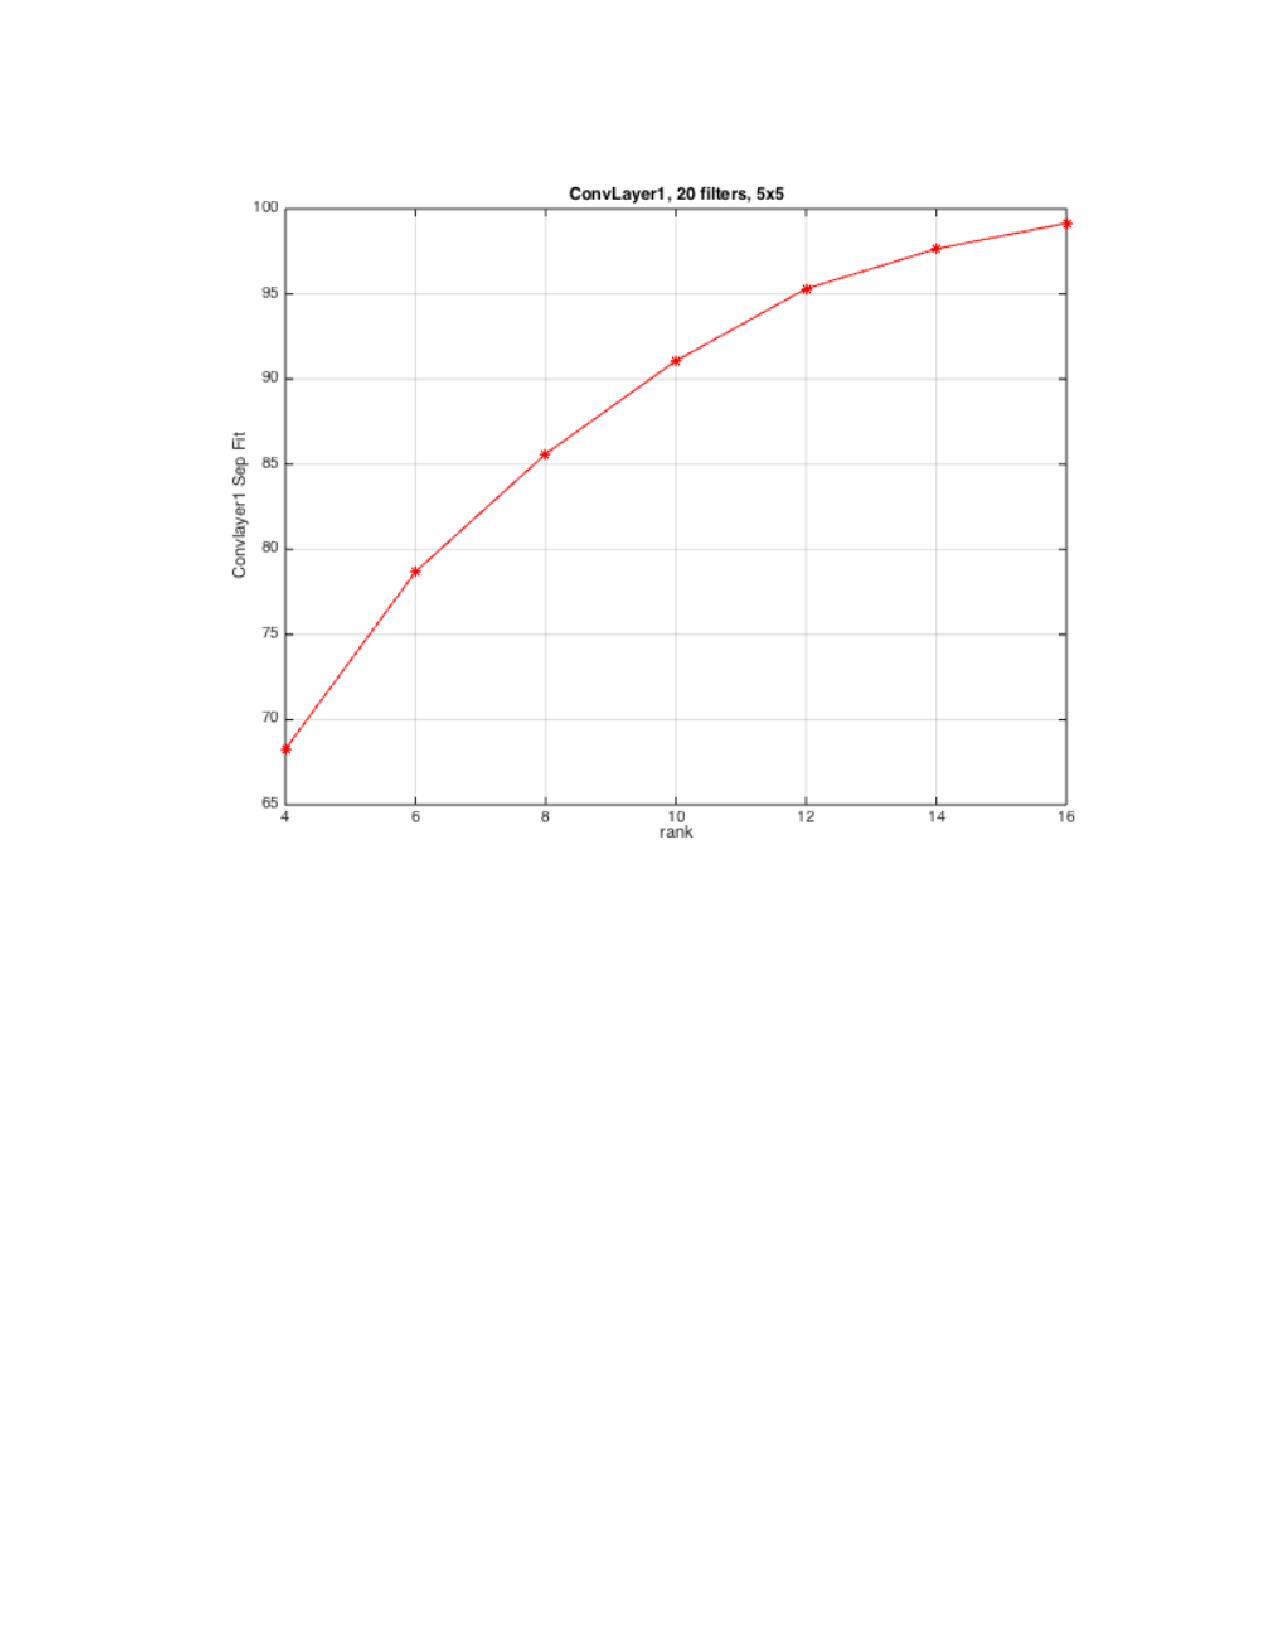
\includegraphics[width=\textwidth]{images/imagesCNN_page6.pdf}
    \caption{Convolutional layer 1}
  \end{subfigure}
  \begin{subfigure}[b]{0.40\textwidth}
    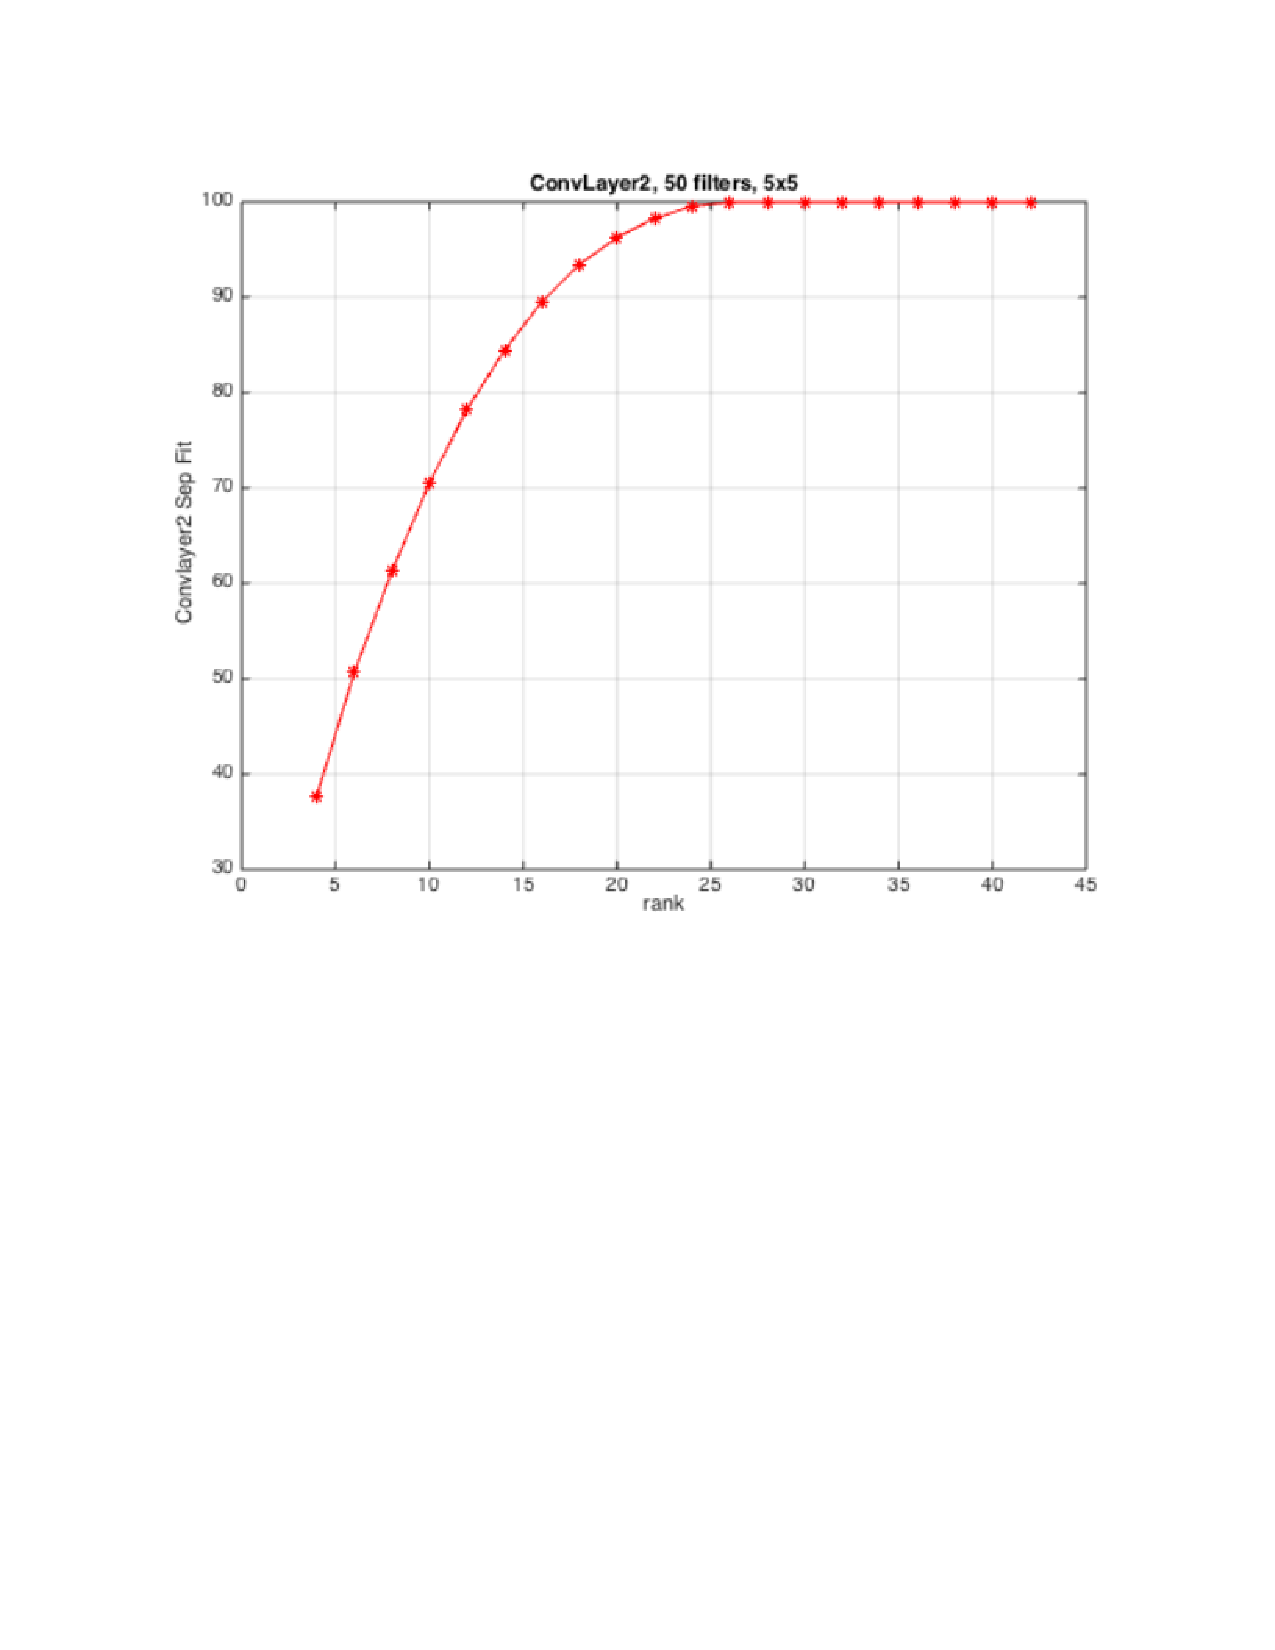
\includegraphics[width=\textwidth]{images/imagesCNN_page2.pdf}
    \caption{Convolutional layer 2}
  \end{subfigure}
  \caption{Rank versus Fit}
  \label{fig:cnn1fitness}
\end{figure}

\begin{figure}[h!]
  \centering
  \begin{subfigure}[b]{0.40\textwidth}
   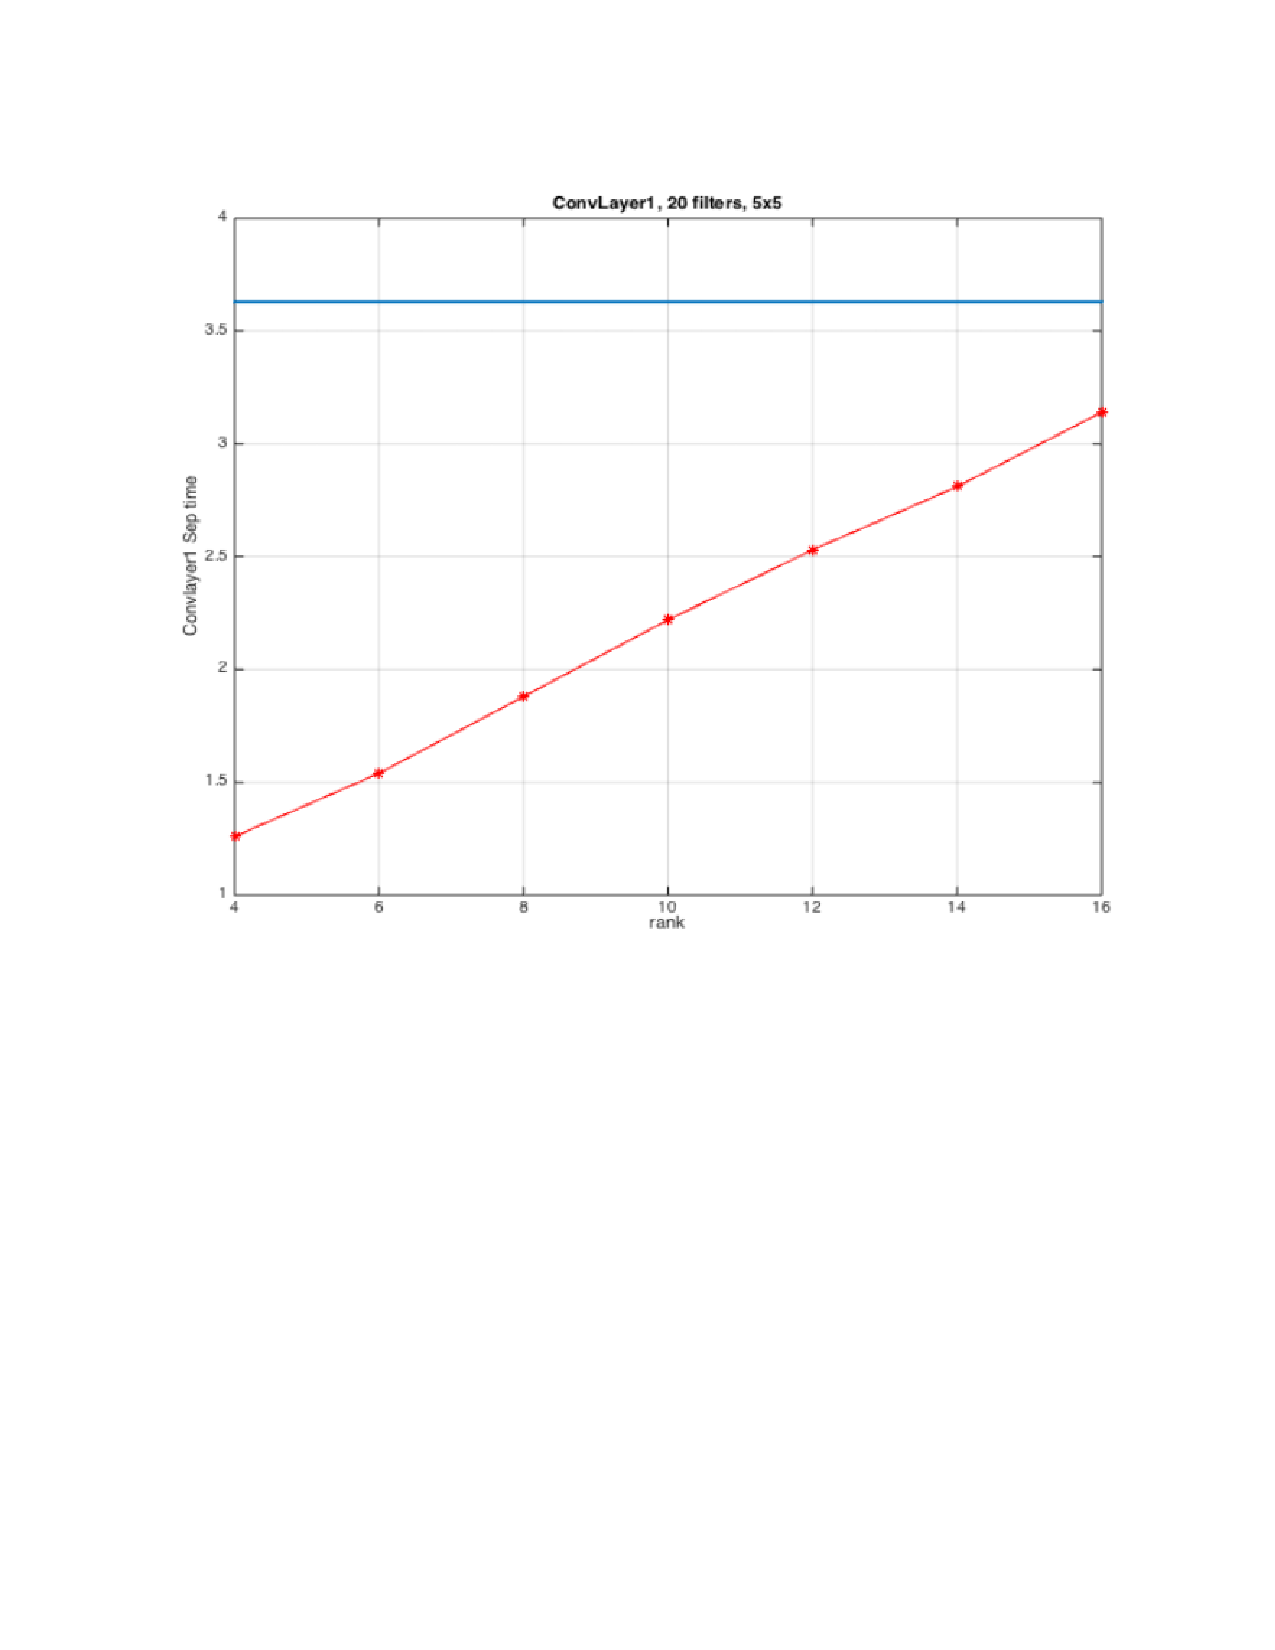
\includegraphics[width=\textwidth]{images/imagesCNN_page5.pdf}
    \caption{Convolutional layer 1}
  \end{subfigure}
  \begin{subfigure}[b]{0.40\textwidth}
    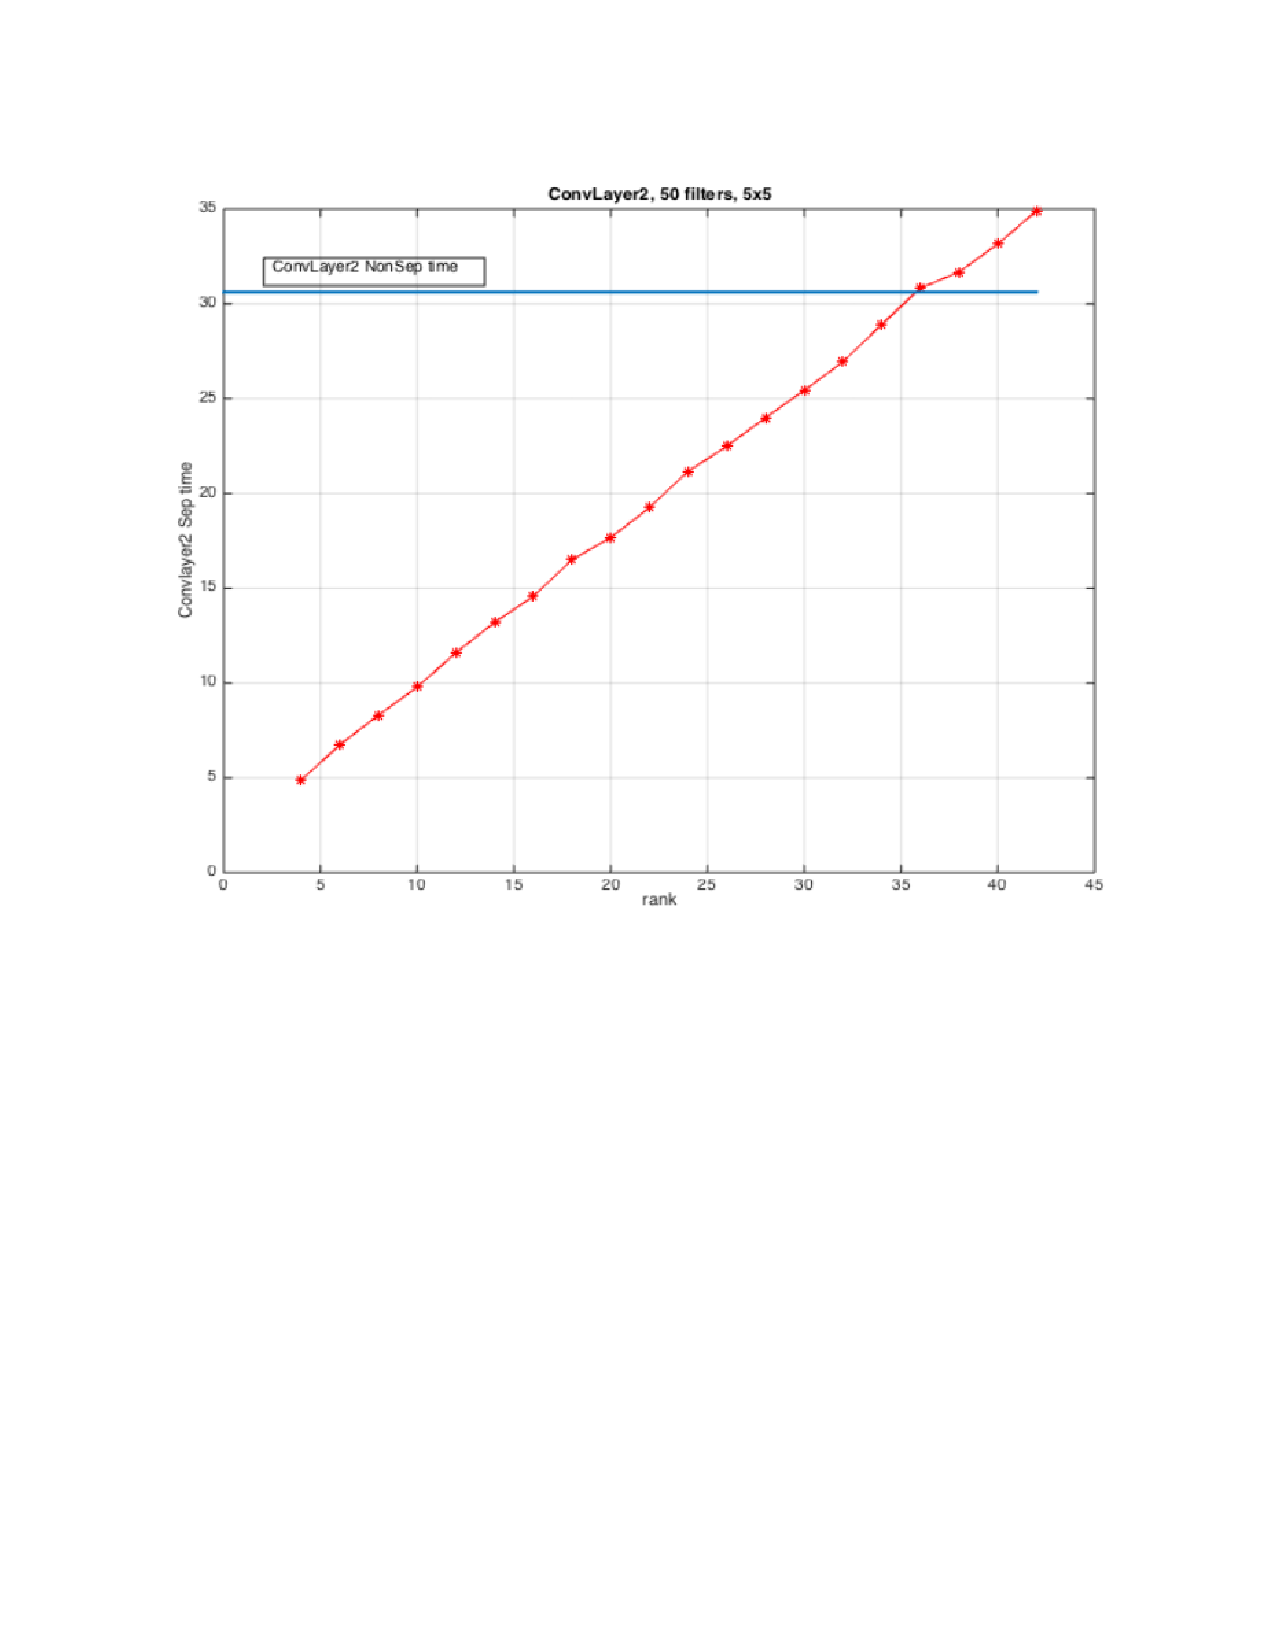
\includegraphics[width=\textwidth]{images/imagesCNN_page3.pdf}
    \caption{Convolutional layer 2}
  \end{subfigure}
  \caption{Rank vs Time}
  \label{fig:cnn1time}
\end{figure}

The question that remains is to see how far we can afford to reduce the rank such that we do not lose much from the classification accuracy. Fig \ref{fig:cnn1error} a shows how the performance of the CNN drops with decreasing rank. With rank 16 the performance is the same, while for rank between 10 and 16 the error rate stays between 0.8 and 0.9 per cent, which is quite low. According to the application, even a rank of 8 or 6 is acceptable, since the drop is not more than 1 per cent.

\begin{figure}[h!]
  \centering
  \begin{subfigure}[b]{0.40\textwidth}
   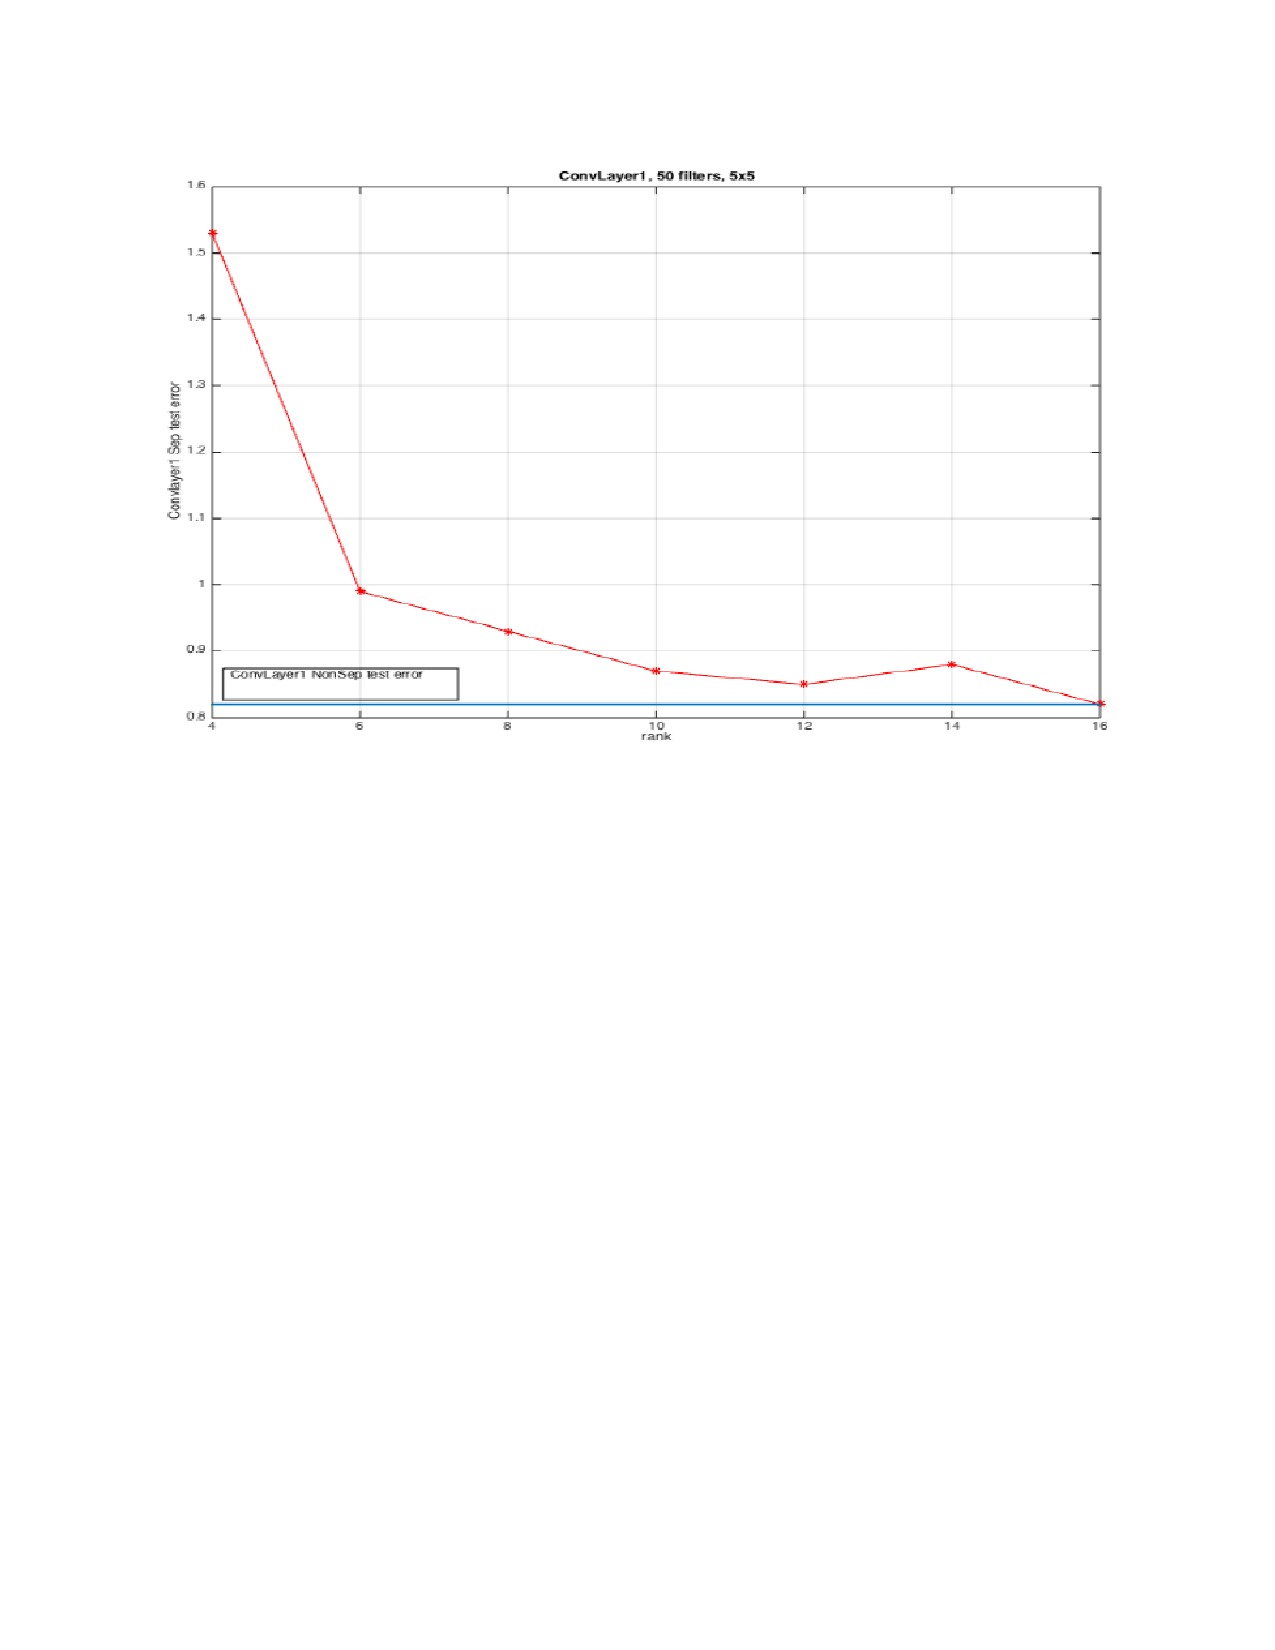
\includegraphics[width=\textwidth]{images/imagesCNN_page4.pdf}
    \caption{Convolutional layer 1}
  \end{subfigure}
  \begin{subfigure}[b]{0.40\textwidth}
    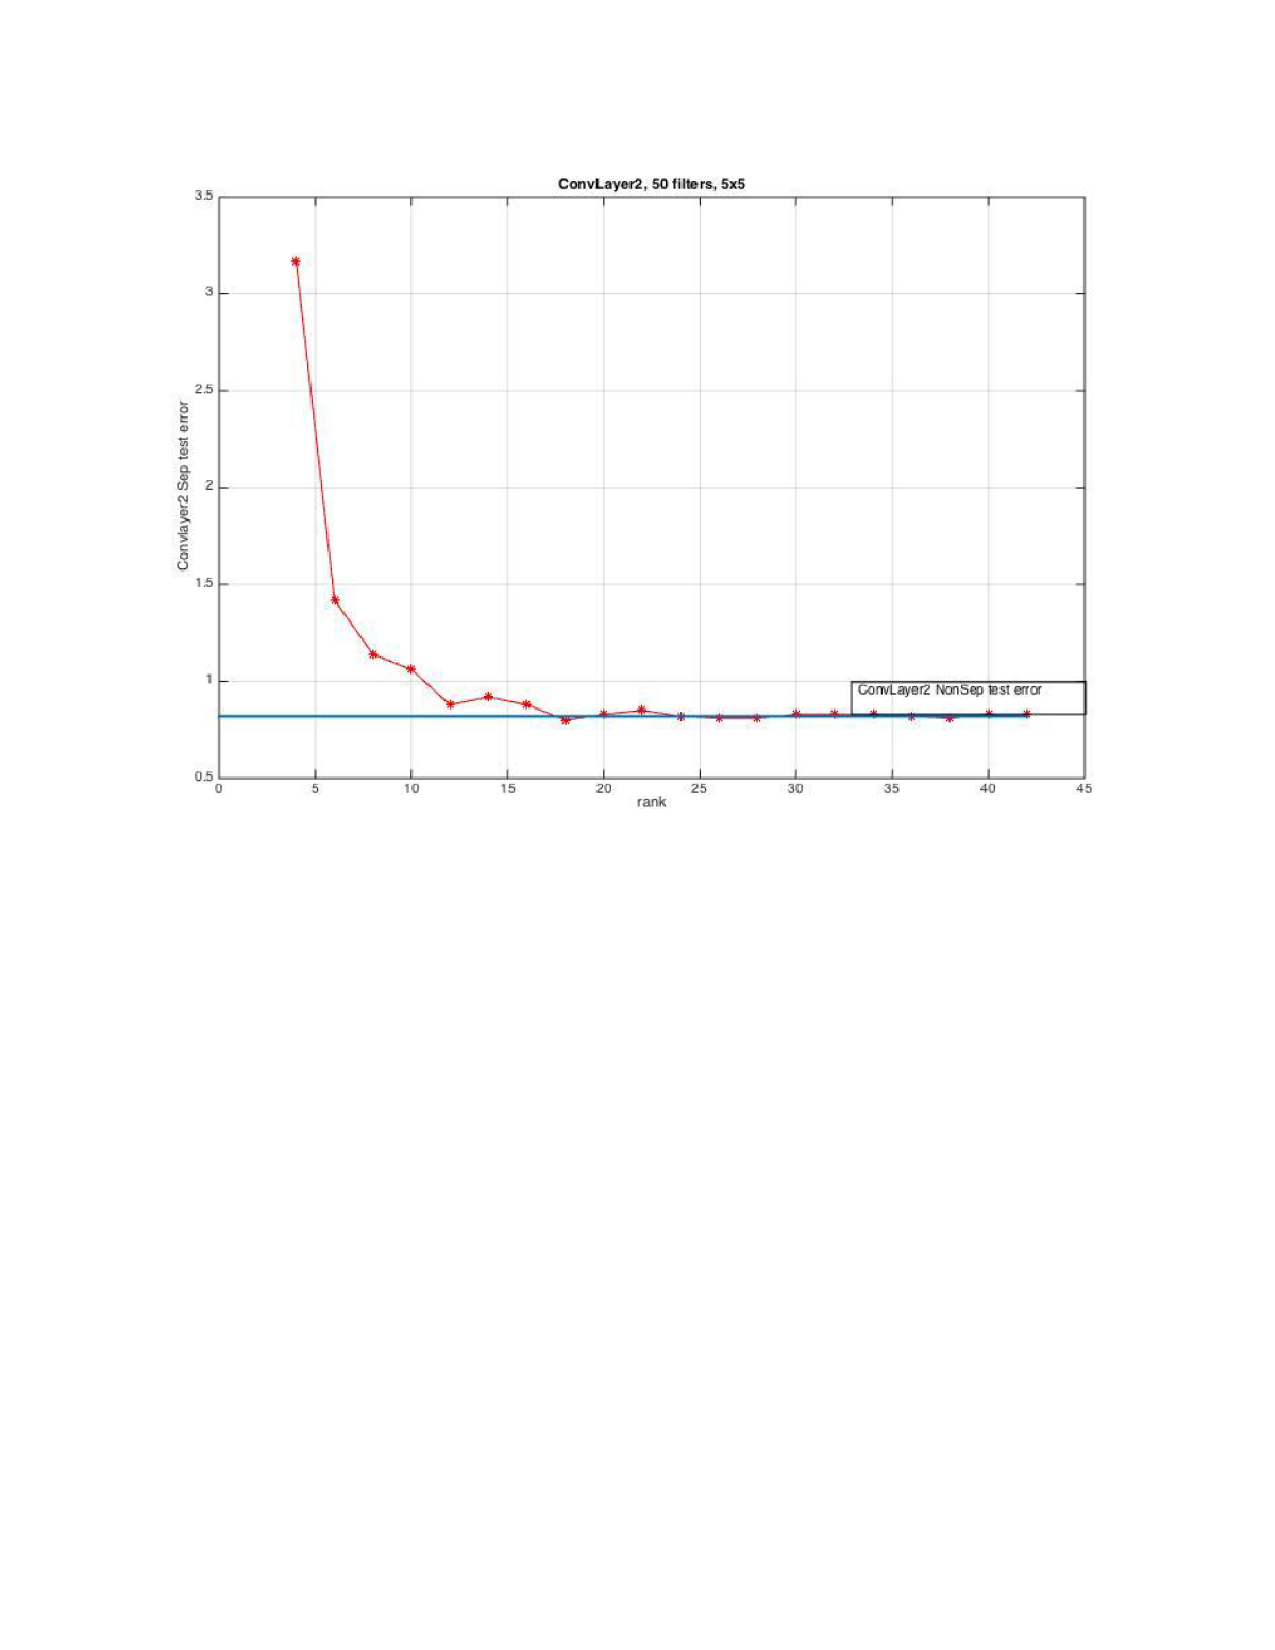
\includegraphics[width=\textwidth]{images/imagesCNN_page1.pdf}
    \caption{}
  \end{subfigure}
  \caption{Convolutional layer 2}
  \label{fig:cnn1error}
\end{figure}

In the second experiment, we kept the first layer unchanged and approximated the second convolutional layer.
Similarly, according to Table \ref{table:rank}, we have a very tall tensor $R^{50\times 5 \times 5}$ with a typical rank of 25.
Fig\ref{fig:cnn1fitness}b shows how well is the approximation with varying rank from 4 to 42 in steps of 2 . As expected, the fit is almost perfect (99.9 fit) for rank higher than the theoretical one of 25.

From the complexity perspective, the separable CNN is faster if we use a rank $K << \frac{Jd_{1}d_{2}}{J +d_{1}+d_{2}} = 20.83$. In our case, for rank = 20 we obtained almost a 40$\%$ speedup. This is due as before to language specific implementation.
For rank 10, using separable filters is actually 3 times faster (theoretically 2 times faster).
If we keep the rank greater than 10, the recognition never drops more than 1 error rate.
For rank 12 the fit is 79 but the error rate is still almost unchanged which means we can easily use rank with relatively bad fit and still obtain good performance. Using separable filters of similar fit of 79  we obtained a slitghly lower performance. This might imply that it is more important to approximate well the first layer, which is the building block for the following layers.
\subsubsection{CNN Model 2}
In the following experiment, we keep the same number of filters per layers but increase the
kernel sizes to $9\times9$ Fig\ref{fig:CNN2}. We obtained a slightly lower performance for this set 1.3 error rate (compared with 0.82 for the previous model). In [cite here \textcolor{red}{find paper}]
they claim that using larger filters does not actually improve peformance of cnns since they struggle to learn bigger filters, but investigating this issue is not the goal of the report.
\begin{table}[h!]
\centering
\begin{tabular}{@{}rlll@{}}\toprule
Layer & Type & Maps and neurons& Kernel size \\ \midrule
0 & input & 1 map of 28x28 &\\
1& convolutional & 20 maps of 24x24 & 9x9\\
2 & max pooling & 20 maps of 12x12 &  \\
3 & convolutional & 50 maps of 8x8& 9x9 \\
4 & max pooling & 50 maps of 4x4&  \\ 
5 & fully conntected& 500 & \\
6 & fully conntected & 2 neurons & \\ \bottomrule
\end{tabular}
\caption{CNN Model 2 for MNIST}
\label{fig:CNN2}
\end{table}
Here we only approximate convolutional layer 2 (rank from 4 to 18 with corresponding fit between 45 and 90). The theoretical rank is less than 49 and we obtain speedup if the rank $K << 59.5$
The results can be seen in Fig\ref{fig:cnn2error}. We notice that up to rank 8 the error of the Separable CNN is reasonable and does not drop more than 1.6 (1.3 is the reference error of the non separable CNN). The speedup for conv L2 drops from 15ms to 12 ms for rank 18 , which is actually much smaller than we expected for using larger filters.
\begin{figure}[h!]
  \centering
  \begin{subfigure}[b]{0.40\textwidth}
   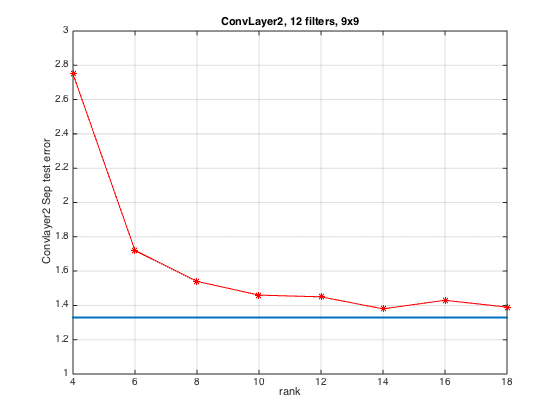
\includegraphics[width=\textwidth]{presentation_plots/convL2_error.png}
    \caption{Error vs Rank}
  \end{subfigure}
  \begin{subfigure}[b]{0.40\textwidth}
    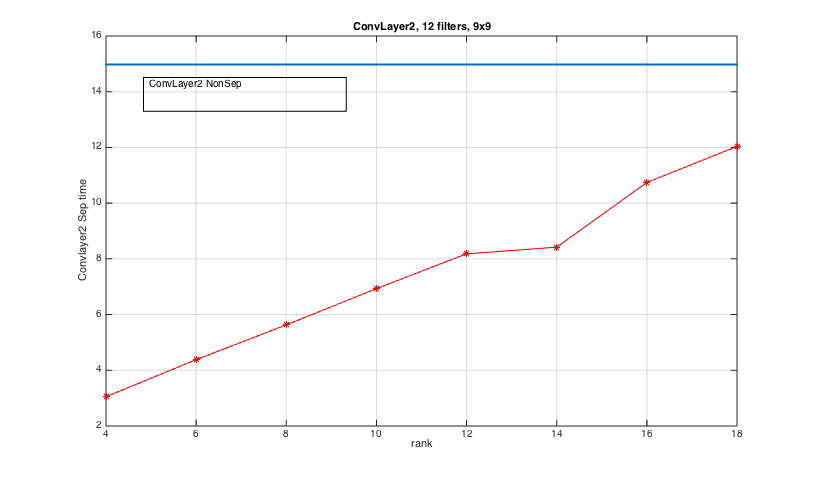
\includegraphics[width=\textwidth]{presentation_plots/convL2_time.png}
    \caption{Rank vs Time}
  \end{subfigure}
  \caption{Convolutional layer 2}
  \label{fig:cnn2error}
\end{figure}
